\documentclass[a4paper,12pt]{report}
\usepackage[T1]{fontenc} % font encodings
\usepackage[utf8]{inputenc} % use utf8 as encoding
\usepackage{lmodern} % use Latin Moderna
\usepackage[french]{babel} % set french as language
\usepackage{graphicx} % manipulate image
\usepackage{hyperref} % use hyper reference
\usepackage{minted} % syntax highlighting
\usepackage{xsim} % exercise helper
\usepackage{titlesec} % manipulate title
\usepackage{xcolor} % manipulate color
\usepackage{enumitem} % better list

\definecolor{bg}{rgb}{0.95,0.95,0.95}
\setminted[java]{breaklines,linenos,autogobble,bgcolor=bg}
\setmintedinline[java]{bgcolor={}}

% remove useless formating of chapter
\titleformat{\chapter}
  {\normalfont\LARGE\bfseries}{\thechapter}{1em}{}
\titlespacing*{\chapter}{0pt}{3.5ex plus 1ex minus .2ex}{2.3ex plus .2ex}

\hypersetup{colorlinks=true}

\xsimsetup{
  exercise/the-counter = \arabic{section}.\arabic{exercise}, % for "Exercice <section>.<number>
  exercise/within = section
}

\begin{document}
\begin{titlepage}
	\centering
	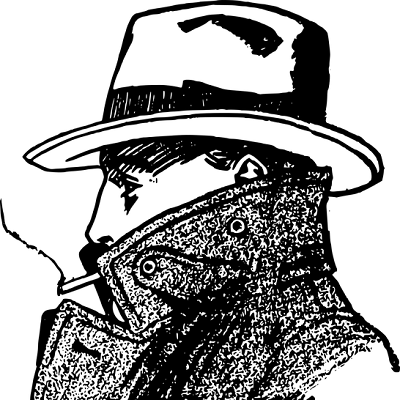
\includegraphics[width=0.15\textwidth]{../media/murphy.png}\\
	\vspace{1cm}
	{\scshape\LARGE ESIEE Paris \\}
	\vspace{2.5cm}
	{\huge\bfseries Rapport projet Zuul\\}
	\vspace{2cm}
	{\Large Corentin POUPRY\\}
	\vfill
	supervisé par\\
	Denis Bureau

	\vfill
	
	{\large 2020 - 2021\\}
\end{titlepage}

\tableofcontents


\chapter{Présentation}

\section{Auteur}

\noindent
Corentin POUPRY, étudiant à l'ESIEE Paris en E1, promotion 2025.

\section{Thème}

\noindent
Murphy Law, un détective, doit faire la lumière sur l'enquête confiée.

\section{Résumé du scénario}

Vous vous attendiez à tomber sur un super jeu de science-fiction proposé par un étudiant talentueux. Cependant, la réalité est tout autre et vous vous retrouvez au bureau d'un curieux détective. Ce détective, bien décidé à vous aider à faire la lumière sur votre cas atypique, c'est Murphy Law, et c'est lui qu'on appelle quand tout va mal.

\section{Scénario détaillé}

Le Joueur (notons la majuscule) est un personnage à part entière de l'histoire, bien que l'utilisateur joue au travers de Murphy Law. Le Joueur apparaît au début de la narration complètement perdu et à la recherche du jeu de science-fiction promis par le talentueux étudiant dans son rapport. Murphy Law, détective, se demande par quel moyen Le Joueur a pu arriver dans son agence alors que, manifestement, il ne fait même pas partie du schéma narratif du jeu. Quelque chose cloche, quelque chose ne tourne pas rond.\\

Murphy Law décide de partir mener l'enquête en allant voir une source pouvant l'aider dans cette enquête. Avec Le Joueur, il monte dans sa voiture (voir \hyperlink{section.1.5}{Plan}), cependant, la structure du jeu commence à se corrompre, à changer dangereusement sans raison, provoquant la stupéfaction chez les deux protagonistes. Murphy accélère pour semer les incohérences de narration. Alors qu'ils roulent vers leur contact à toute allure, Murphy commence à perdre le contrôle de la situation jusqu'à qu'un arbre apparaisse devant la voiture provoquant un accident.\\

Murphy Law et Le Joueur se réveille dans la pénombre d'un hangar inconnue, peu après, une explosion se fait ressentir et une alerte rouge se déclenche. En sortant du hangar, les protagonistes se rendent compte qu'ils sont sur l'USS Enterprise de l'Univers Star Trek, en pleine bataille.\\

Alors que Le Joueur et Murphy Law referme le SAS en vitesse derrière eux, ils se retrouvent dans le salon de réception de Buckingham Palace. 

Puis La pyramide ou Le Joueur et Murphy sont séparés.\\

Après avoir perdu le joueur et flairant que quelque chose se trame dans son dos, Murphy Law décide alors de se rendre là où tout a commencé : dans la salle de l'ESIEE où Le Joueur avait lancé le jeu. S'en suit une confrontation avec Le Compilateur, qui essayait de manipuler le jeu à sa guise. Murphy en ressort gagnant.\\

\section{Plan}

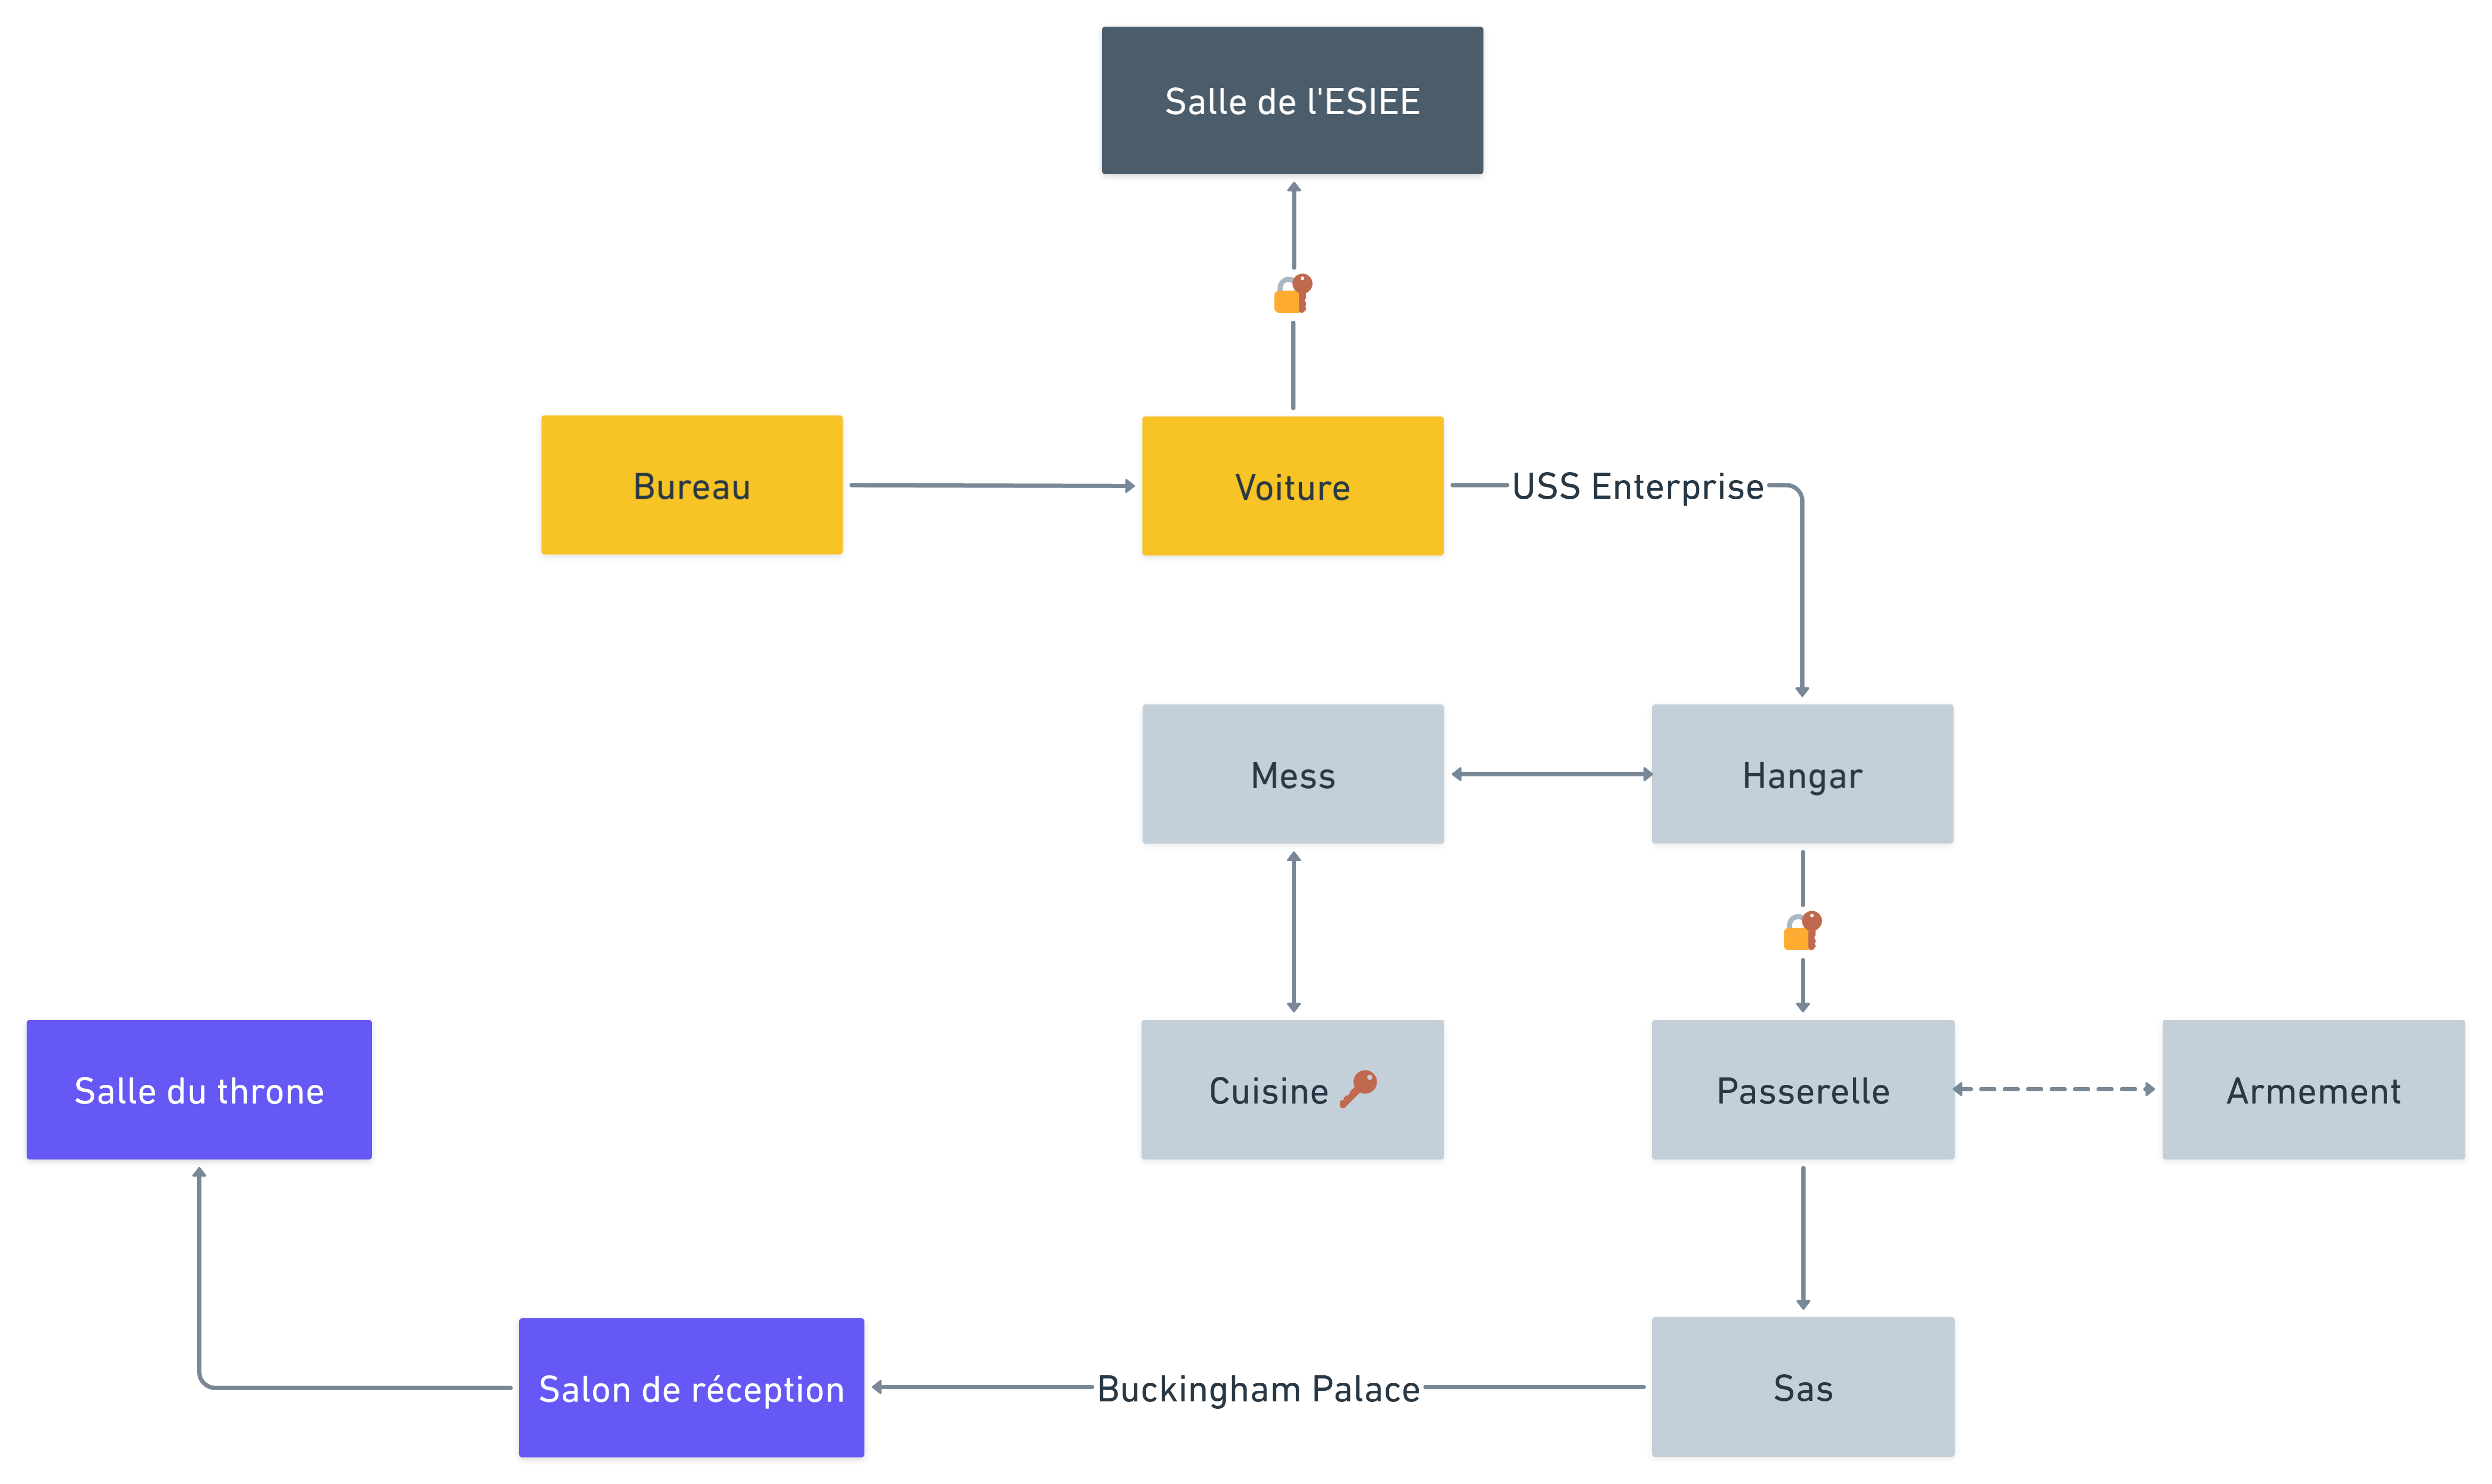
\includegraphics[width=\textwidth,height=\textheight,keepaspectratio]{../media/map.png}\\

\section{Détail des lieux, items, personnages}

\subsection{Lieux}

\begin{description}[leftmargin=!,labelwidth=\widthof{\bfseries Bureau de Murphy}]
  \item [Bureau de Murphy] C'est le lieu où vous commencez votre aventure.
  \item [Salle de l'ESIEE] C'est dans cette salle de l'ESIEE que vous avez lancé ce jeu.
\end{description}

\subsection{Personnages}

\begin{description}[leftmargin=!,labelwidth=\widthof{\bfseries Le Compilateur}]
  \item [Murphy Law] Le détective et le personnage que vous incarnez. Son rôle est de mener l'enquête pour comprendre par quelles circonstances Le Joueur s'est retrouvé ici.
  \item [Le Narrateur] La voix que vous entendez quand vous jouez. Le Narrateur permet de décrire les scènes \& situations sans sortir de la narration. 
  \item [Le Joueur] C'est vous ! Cependant, Le Joueur est paradoxalement un personnage non jouable qui vous représente tout au long de  l'histoire dans le cadre de la méta-narration.
  \item [Le Compilateur] Le compilateur Java est le grand méchant de l'histoire. Son rôle, manipuler la structure du jeu pour que l'étudiant n'ait pas une note à la hauteur de son travail.
\end{description}

\section{Situations gagnantes et perdantes}

Le Joueur et Murphy Law seront confrontés à des situations de crises où des choix et décisions devront être prises, certains pourront entraîner la mort des protagonistes et donc faire gagner Le Compilateur.\\
La liste des situations perdantes est la suivante :

\begin{description}[align=left,leftmargin=!,labelwidth=\widthof{\bfseries A Buckingham Palace}]
  \item [Sur l'USS Enterprise]
  \item [Dans la pyramide]
  \item [A Buckingham Palace] 
\end{description}

\section{Commentaires}

Murphy Law est une création originale de \href{http://scp-wiki.wikidot.com/murphy-law-hub}{la Fondation SCP}. Le personnage, les œuvres associées et ce jeu sont tous proposés sous licence \emph{Creative Commons Attribution-ShareAlike 3.0}


\chapter{Exercices}

% The first really interesting exercise to write is 7.5. 
% We initialize our counters to match this situation.
\setcounter{section}{7}
\setcounter{exercise}{4}


\begin{exercise}[subtitle=printLocationInfo]

En ré-usinant le code de l'affichage de la localisation et des sorties en une fonction, on s'assure de ne pas répéter cette partie à plusieurs endroits.

\begin{minted}{java}
private void printLocationInfo() {
    Room vCurrent = this.aCurrentRoom;
    System.out.printf("You are %s%n", vCurrent.getDescription());
   
    System.out.print("Exits: ");
    if (vCurrent.aEastExit != null) System.out.print("east ");
    if (vCurrent.aNorthExit != null) System.out.print("north ");
    if (vCurrent.aSouthExit != null) System.out.print("south ");
    if (vCurrent.aWestExit != null) System.out.print("west ");
    System.out.println();
}
\end{minted}

\end{exercise}

\vfill

\begin{exercise}[subtitle=getExit]

Dans cet exercice, on se rend compte que le système "un attribut = une sortie" n'est pas le plus optimal (imaginons un hub ayant une dizaines de sorties par exemple, ce qui deviendrait problématique pour la lisibilité et la maintenance du code). L'idée étant de limiter le couplage entre la classe \verb|Room| et les autres classes. Pour cela, on cherchera à limiter la dépendance aux attributs de Room et plutôt passer par une fonction pour récupérer les sorties, ce qui permet de ne pas avoir à se soucier de l'implémentation du côté de \verb|Room|.\\ 

\textbf{Notes:} Notons qu'il reste un problème dans \verb|printLocationInfo| à cause de ce changement.

\vfill

\begin{minted}{java}
/**
 * Retrieves the Room associated with the exit
 * in the requested direction.
 * @param pDirection the direction of the exit.
 * @return the room associated with the exit.
 */
public Room getExit(final String pDirection) {
    switch (pDirection) {
        case "north":
            return this.aNorthExit;

        case "east":
            return this.aEastExit;

        case "south":
            return this.aSouthExit;

        case "west":
            return this.aWestExit;

        default:
            return null;
    }
}
\end{minted}

\end{exercise}

\vfill

\begin{exercise}[subtitle=getExitString]
Le dernier changement a impacté la façon dont \verb|printLocationInfo| fonctionne. Pour le résoudre, on écrit une nouvelle méthode \verb|getExitString| et, fort de ce changement, on ré-usine \verb|printLocationInfo|.

\begin{minted}{java}
/**
 * Gets all existing exits.
 * @return a string with the possibles exits.
 */
public String getExitString() {
    String vResult = "Exits: ";

    if (this.aEastExit != null) vResult += "east ";
    if (this.aNorthExit != null) vResult += "north ";
    if (this.aSouthExit != null) vResult += "south ";
    if (this.aWestExit != null) vResult += "west";

    return vResult;
}

/**
 * Prints the location informations.
 */
private void printLocationInfo() {
    Room vCurrent = this.aCurrentRoom;

    System.out.printf("You are %s%n", vCurrent.getDescription());
    System.out.println(vCurrent.getExitString());
}
\end{minted}
\end{exercise}

\begin{exercise}[subtitle=HashMap et setExit]

Maintenant que le couplage entre \verb|Room| et \verb|Game| est faible, on peut remplacer les détails de l'implémentation sans risquer de casser quelque chose. On utilise une structure de données \verb|HashMap| et on doit changer les méthodes de \verb|Room| en conséquence. On en profite aussi pour remplacer \verb|setExits|, devenue inutile, par \verb|setExit|.

\vfill

\begin{minted}{java}
/**
 * Set an exit of the room
 * @param pDirection the direction of the exit
 * @param pExit the Room to which the exit leads
 */
public void setExit(final String pDirection, final Room pExit) {
    this.aExits.put(pDirection, pExit);
}

/**
 * Retrieves the Room associated with the exit in the requested direction.
 *
 * @param pDirection the direction of the exit.
 * @return the room associated with the exit.
 */
public Room getExit(final String pDirection) {
    return this.aExits.get(pDirection);
}
\end{minted}
\end{exercise}

\begin{exercise}[subtitle=keySet]

\verb|getExitString| doit elle aussi être modifiée. Plutôt que de tester la présence de certaines valeurs dans la \verb|HashMap| (du type "north", "east", "down", "up"...), on peut énumérer les différentes clés qui composent la \verb|HashMap| des sorties.

\begin{minted}{java}
/**
 * Gets all existing exits of the room.
 *
 * @return a string with the possibles exits.
 */
public String getExitString() {
    String vResult = "Exits : ";
    for (String vExit : this.aExits.keySet())
        vResult += vExit + " ";

    return vResult;
}
\end{minted}
\end{exercise}

\begin{exercise}[subtitle=Fonctionnement de keySet]

Reprenons le code intéressant de l'exercice précédent et intéressons-nous à son fonctionnement.

\begin{minted}{java}
for (String vExit : this.aExits.keySet())
    vResult += vExit + " ";
\end{minted}

D'après la documentation Java, \mintinline{java}{.keySet()} retourne un \verb|Set<K>| miroir contenant les clefs de \verb|HashMap<K, V>| (ici notre \verb|HashMap| étant  \mintinline{java}{this.aExits}). Maintenant, si on s'intéresse a l'interface \verb|Set|, on voit qu'elle repose elle-même sur plusieurs interfaces, notamment \verb|Iterable<K>|, lui donnant la possibilité de s'utiliser dans une boucle for-each.

\end{exercise}

\chapter{Mode d'emploi}

\chapter{Plagiat}

\end{document}
